De acordo com um relat�rio recente da Ag�ncia Internacional de Energia (AIE), o mercado de ve�culos el�tricos atingiu um novo marco em 2016, quando foram vendidos mais de 750 mil autom�veis da categoria. Com isso, o total de carros el�tricos vendidos no mundo alcan�ou a marca de 2 milh�es de unidades desde que os primeiros modelos come�aram a ser comercializados em 2011. 
No Brasil, a expans�o das vendas tamb�m se verifica. A marca A, por exemplo, expandiu suas vendas no ano de 2016, superando em 360 unidades as vendas de 2015, conforme representado no gr�fico. 

\begin{figure}[h]
\centering
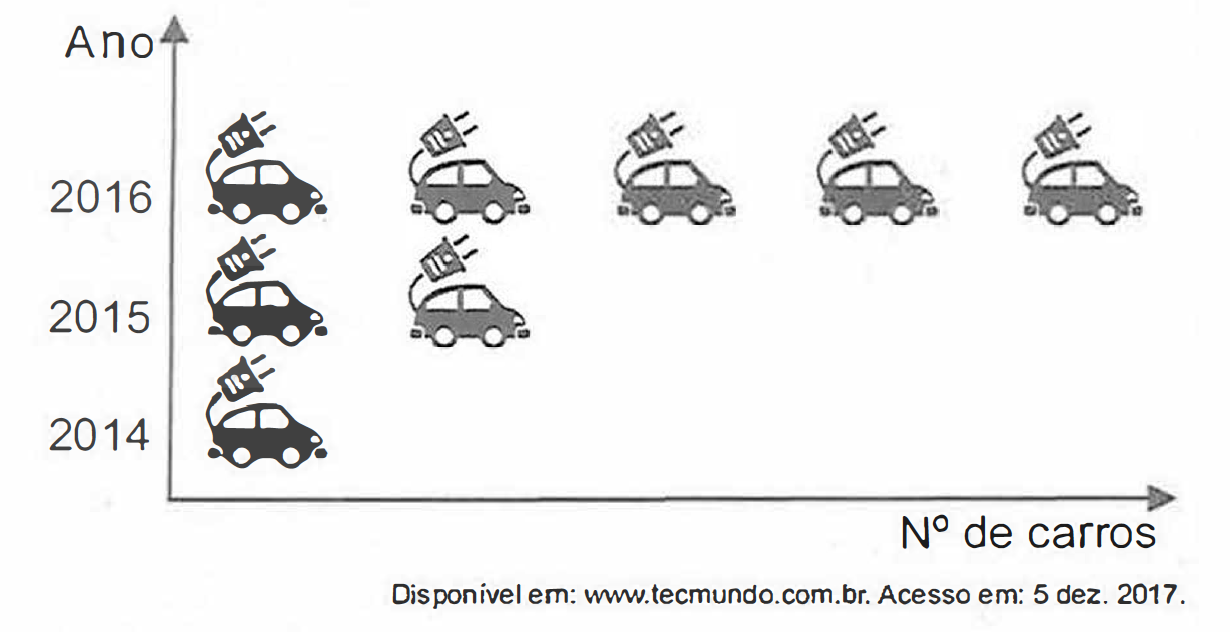
\includegraphics[width=8cm]{../figuras/q177-2018.png}
\end{figure}

A m�dia anual do n�mero de carros vendidos pela marca A, nos anos representados no gr�fico, foi de 

\begin{enumerate}
\item[a)]192
\item[b)]240
\item[c)]252
\item[d)]320
\item[e)]420
\end{enumerate}